%!TEX root = report.tex
\subsection{Experimental Results}

\subsubsection{Performance measure}
The performance of the localization can be quantified in terms of the distance from the calculated target point to its real position (measured with laser pointer). 
Both algorithms with fixed height and free height respectively (see § \ref{sec:triangulation} are applied and the errors in the x-y plane (for fixed height and free height) as well as the 3D error (for free height) are considered. 

It was found that the error of the robot depends a lot on which cameras are used for triangulating the image points. 
Since in a later experimental setup, the real position of the robot should not be measured anymore, it is not imminent how the best camera combination can be found. 
It was considered to determine it using the respective errors of the reprojection of the reference points, whose positions are well known. 
However, the results in Figure \ref{fig:res0_err} suggest that there is no strong enough correlation between the reference point error and the robot error, which is why a different criterion needs to be found. 
This exceeds the scope of the present project, so in the following considerations, all camera combinations and the real position of the robot are used for measurement of performance. 

\begin{figure}[H] 
    \centering
    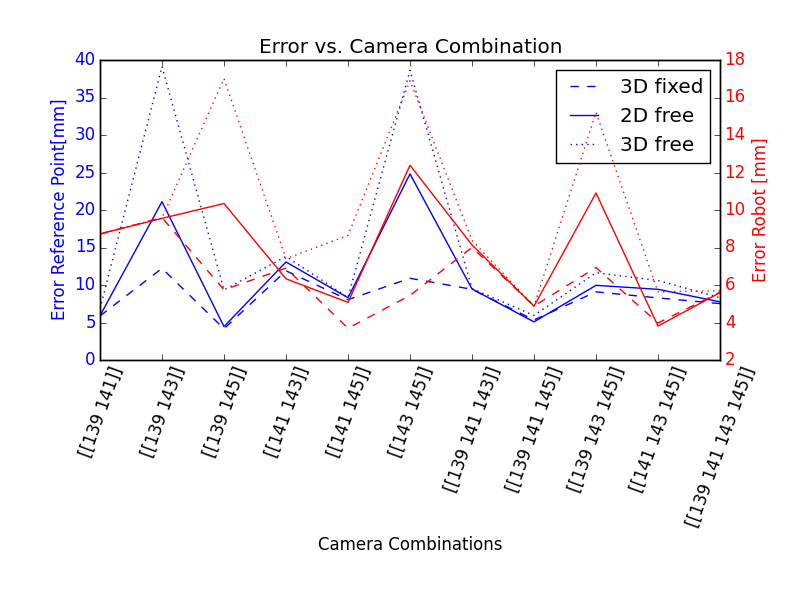
\includegraphics[width=.8\linewidth]{files/res0_combi_4.png}
    \caption{Results of experiment in Atrium}
    \label{fig:res0_err}
\end{figure}

\subsubsection{Reference frames}
Two reference frames are used in the experiments: First, there is the reference point frame, in which the visual localization is done. 
In this frame, the x axis is defined to point from the first to the second reference point (\textit{ref basis} in Figure \ref{fig:res1_room} and \ref{fig:res2_room} ) and the y axis points from the first point to where the other points are.
For visualization, a margin in x and y direction is added to these points, so the origin is slightly offset from the basis line (see \textit{ref origin} in Figures \ref{fig:res1_room} and \ref{fig:res2_room}).

\subsubsection{Atrium}
The first experiments were done in the Atrium of the BC building, with 5 orange reference points for extrinsic calibration and a bottle as a target point instead of the robot.
This setup is characterized by no big height difference between the reference points (height 20 mm) and the target point (height 160 mm). 
The cameras are placed at a height of around 2 meters which leads to bottom-down views for all cameras (Figure \ref{fig:res0_img139} and \ref{fig:res0_img141}).
The resulting error of the robot position is less than 18mm for all camera combinations and goes down to 5.8mm in 3D (139,141,145) or 4 mm in 2D with fixed height (139,143). 
\begin{figure}[H]
    \centering
    \begin{subfigure}{0.49\linewidth}
        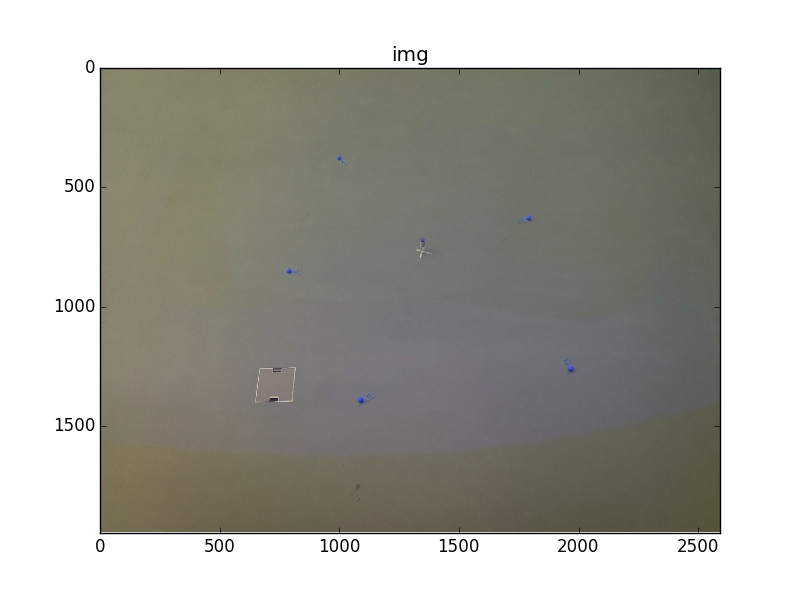
\includegraphics[width=\linewidth]{files/res0_img139.png}
        \caption{View of camera 139 }
        \label{fig:res0_img139}
    \end{subfigure}
    \begin{subfigure}{0.49\linewidth}
        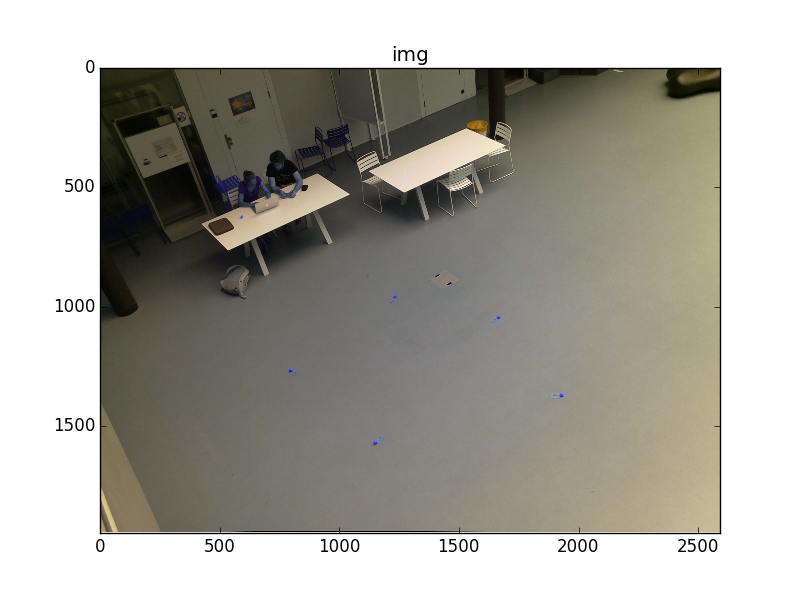
\includegraphics[width=\linewidth]{files/res0_img141.png}
        \caption{View of camera 141 }
        \label{fig:res0_img141}
    \end{subfigure}
    \caption{Camera views of experiment in Atrium}
    \label{fig:res0_views}
\end{figure}


\subsubsection{BC329 with reference points}

A second experiment was performed in a more realistic setting, using 6 reference points for extrinsic calibration and the real robot as target point (see Figure \ref{fig:res1_img}). 
\begin{figure}[H]
    \centering
    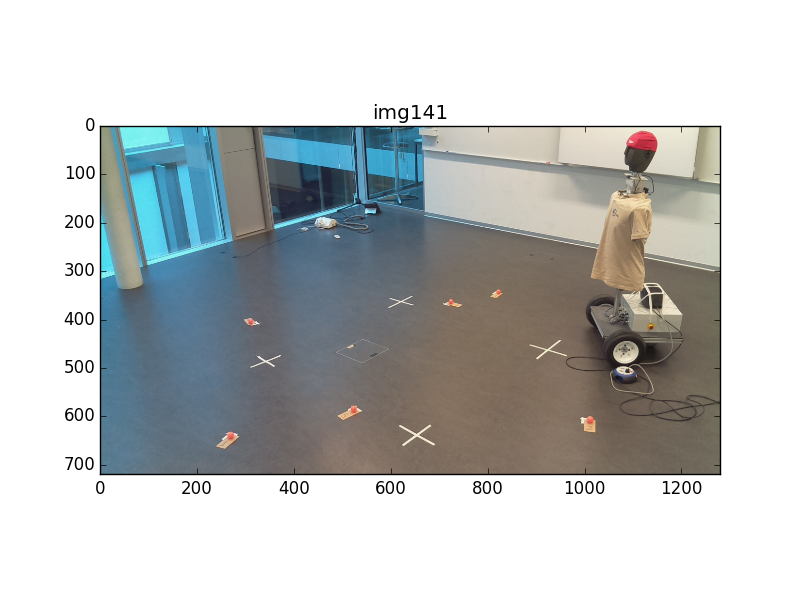
\includegraphics[width=.6\linewidth]{files/res1_img141.png}
    \caption{View of camera 141}
    \label{fig:res1_img}
\end{figure}
The results of the visual localization were compared to the robot's \"own\" perception using odometry and the camera positions where also recorded.
The performance of odometry could be measured at 3 positions but because of technical issues, only one visual localization could be performed. 
The robot's real positions, ad measured positions within the room and the placement of the cameras are visualized in Figure \ref{fig:res1_room}.
The visual localization is quite off the real positions, which can be more clearly seen in Figure \ref{fig:res1_combi}. 

\begin{figure}[H]
    \centering
    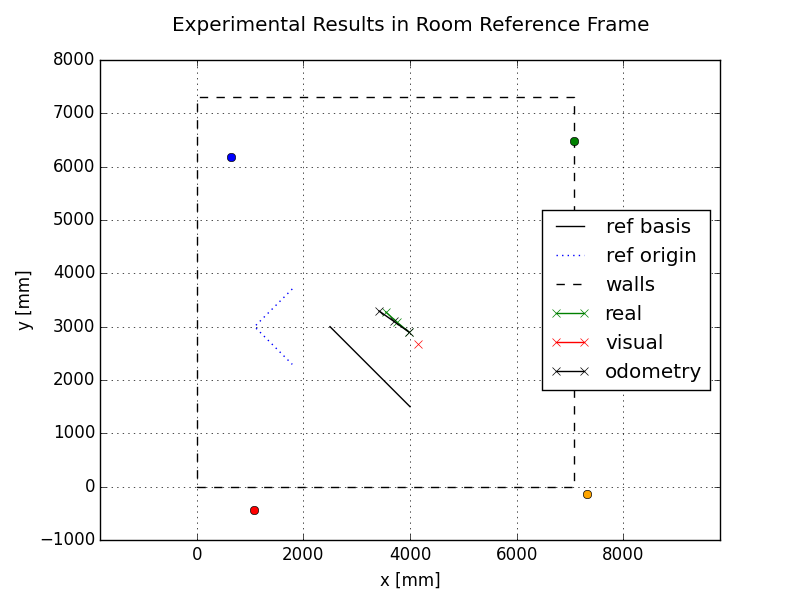
\includegraphics[width=.8\linewidth]{files/res1_room.png}
    \caption{Results of experiment 1 in BC329 (Camera numbering: blue 139, red 141, green 143, orange 145).}
    \label{fig:res1_room}
\end{figure}

The best result is obtained with the combination (141,143), all other results being significantly higher. 
The resulting error (46 mm) is significantly higher than in the Atrium, as the view is much less bottom-down, so little errors in height lead to big lateral errors.
A more closer look of the results reveils that the height of the robot is very badly determined when camera 145 is used. This doesn't show in the positioning of the camera, which is as accurate as the others (Figure \ref{fig:res1_room}, orange point). 
It could be that its relative position to the robot might be poorly chosen, as it is relatively close to the robot head and little errors in height lead to a very big lateral error. (see Figure \ref{fig:res1_img145})

\begin{figure}[H]
    \centering
    \begin{subfigure}{0.49\linewidth}
        \centering
        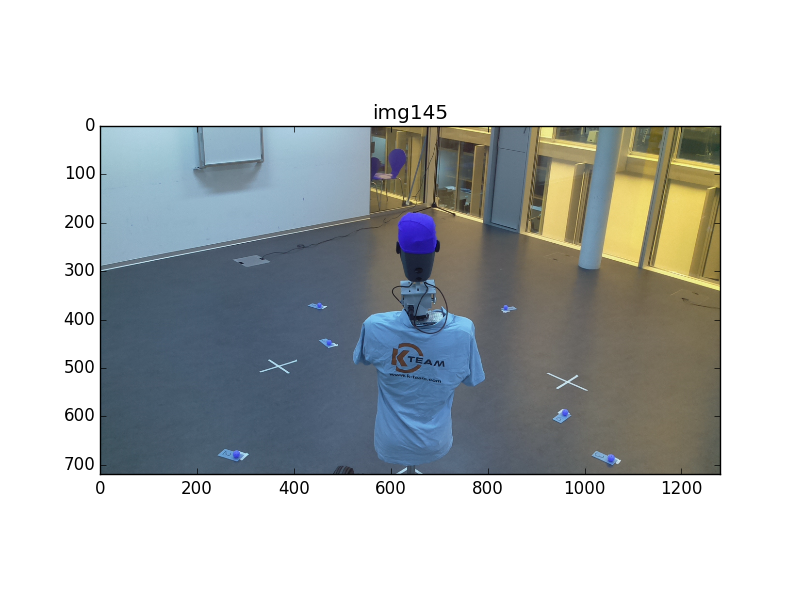
\includegraphics[width=\linewidth]{files/res1_img145.png}
        \caption{View of camera 145}
        \label{fig:res1_img145}
    \end{subfigure}
    \begin{subfigure}{0.49\linewidth}
        \centering
        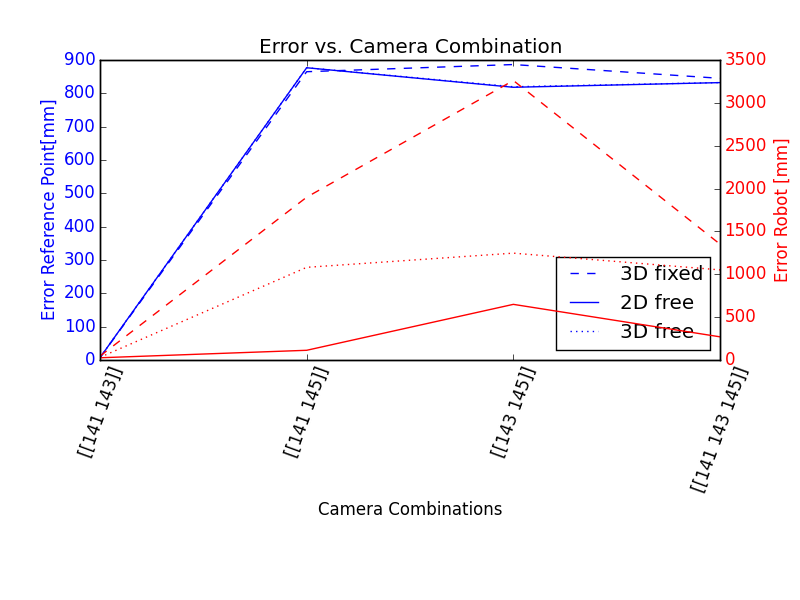
\includegraphics[width=\linewidth]{files/res1_combi_4.png}
        \caption{2D and 3D errors of 4th reference point and robot at the first position}
        \label{fig:res1_combi}
    \end{subfigure}
    \caption{Results of experiment 1 in BC329}
    \label{fig:experiment1}
\end{figure}



\subsubsection{BC329 with checkerboard}

A third experiment was performed in the same setting but using the checkerboard algorithm for extrinsic calibration (see Figures \ref{fig:res2_image_143} and  \ref{fig:res2_image_145}). 
The visual localization was done at two locations and its results were significantly better than for the first experiment. 

\begin{figure}[H]
    \centering
    \begin{subfigure}{0.49\linewidth}
        \centering
        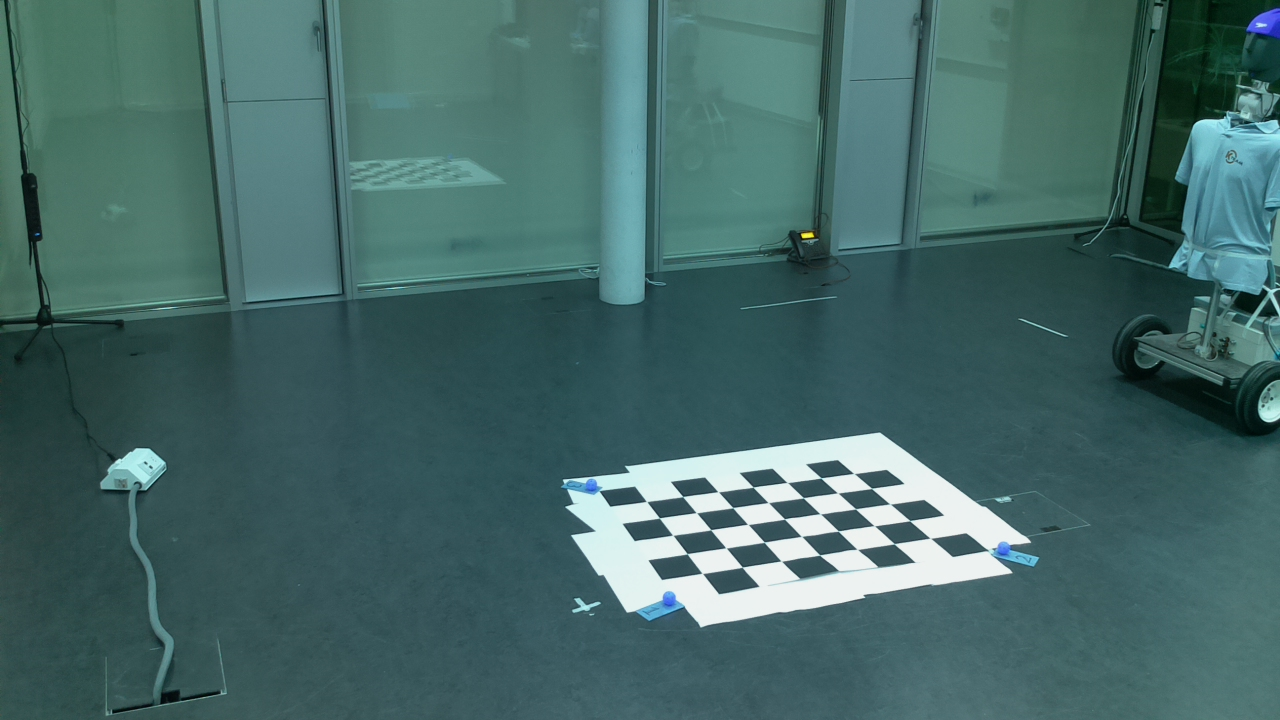
\includegraphics[width=\linewidth]{files/res2_image_143.png}
        \caption{Camera 143}
        \label{fig:res2_image_143}
    \end{subfigure}
    \begin{subfigure}{0.49\linewidth}
        \centering
        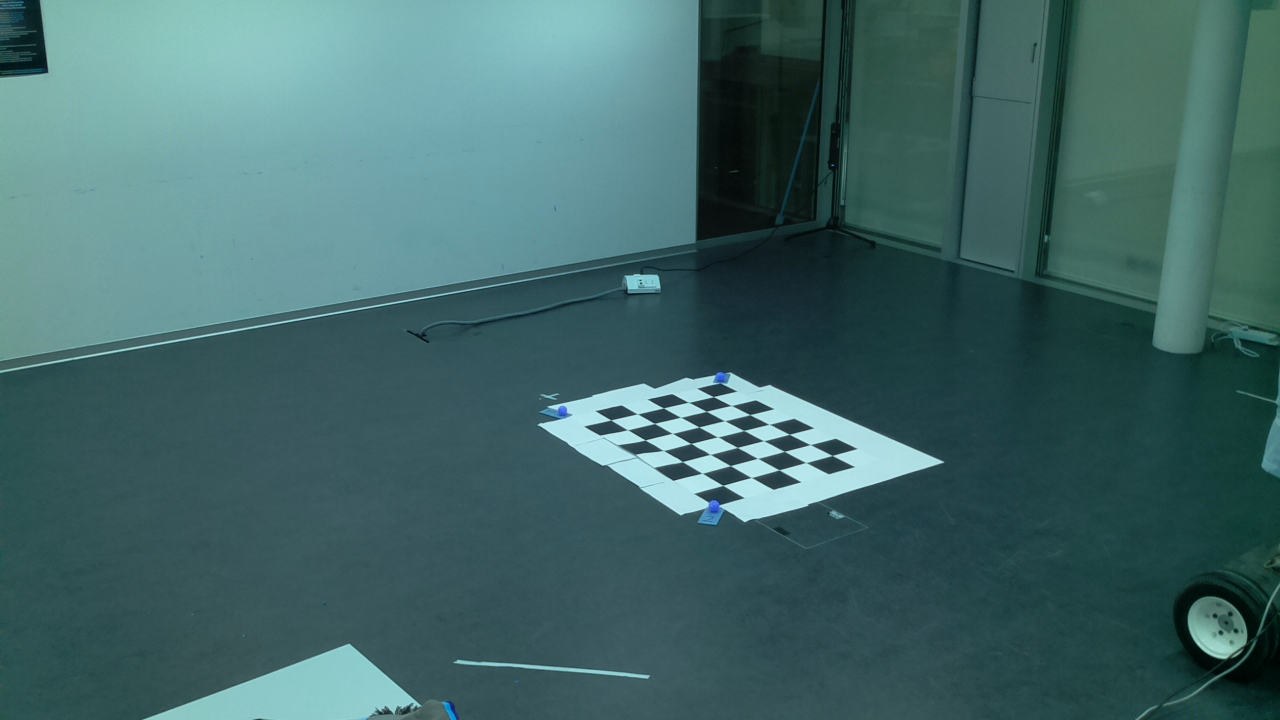
\includegraphics[width=\linewidth]{files/res2_image_145.png}
        \caption{Camera 145}
        \label{fig:res2_image_145}
    \end{subfigure}
    \caption{Camera views for extrinsic calibration in BC329}
    \label{fig:experiment1}
\end{figure}

The robot position errors are shown in Figure \ref{fig:res2_combi}. Two tendencies can be observed: 
Including the camera 145 tends to spoil the result, whereas an increasing number of cameras tends to improve the result. The best result is obtained for the combination (141,143,145) of an error of around 80mm.
For the second position, only cameras 139 and 141 could be considered because of technical issues and they led to an error of around 100mm both fixed and free. 
\begin{figure}[H]
    \centering
    \begin{subfigure}{0.49\linewidth}
        \centering
        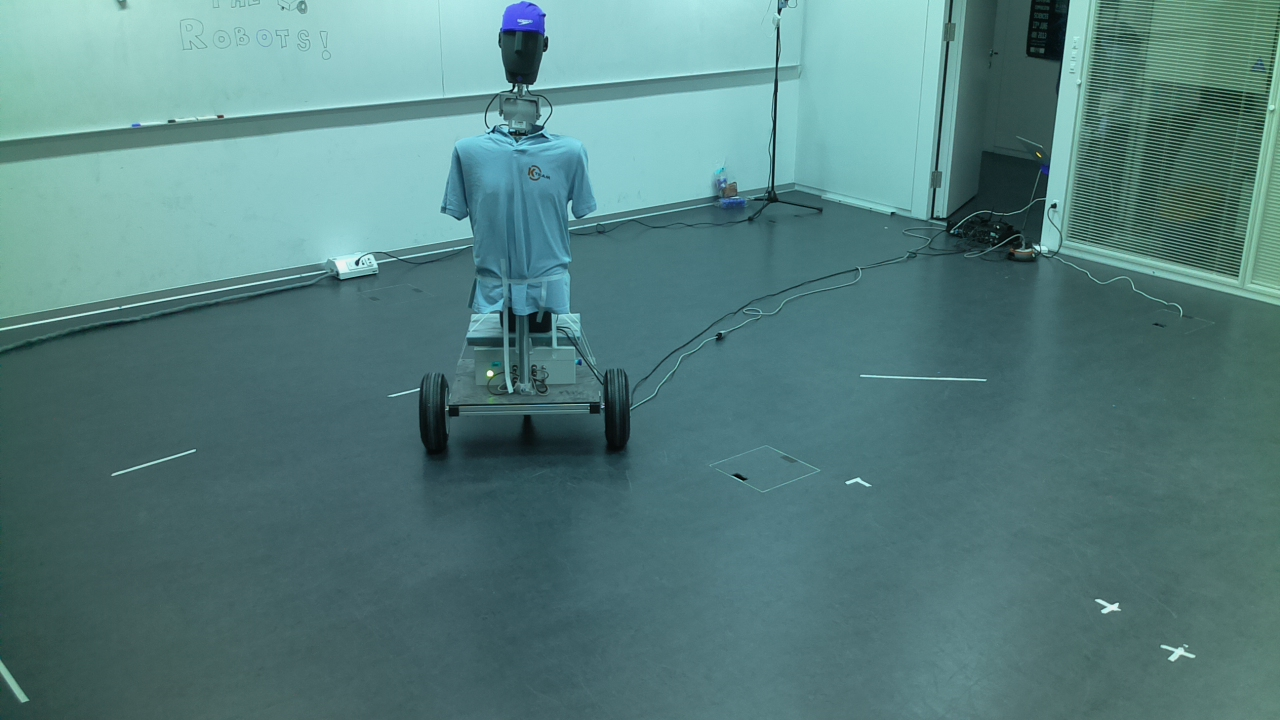
\includegraphics[width=\linewidth]{files/res2_0_image_141.png}
        \caption{View of camera 141 with robot}
        \label{fig:res2_0_image_141}
    \end{subfigure}
    \begin{subfigure}{0.49\linewidth}
        \centering
        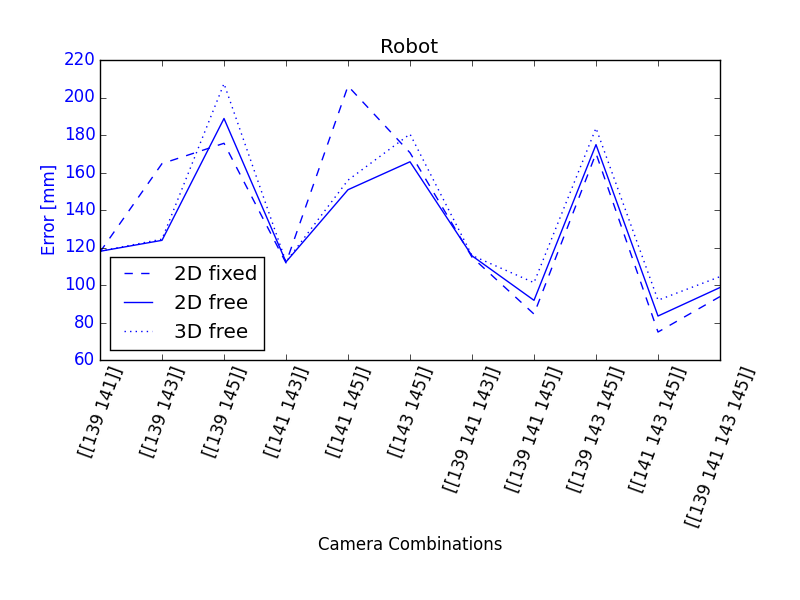
\includegraphics[width=\linewidth]{files/res2_combi_rob.png}
        \caption{2D and 3D errors of robot}
        \label{fig:res2_combi}
    \end{subfigure}
    \caption{Results of experiment 2 in BC329 }
    \label{fig:experiment1}
\end{figure}
In general, the height was very accurately determined with 1615mm at the first position and 1640mm at the second position (Table \ref{tab:res2_errors}).
The results and the camera positions are shown in Figure \ref{fig:res2_room}.

\begin{table}[H]
\begin{center}
\caption{Obtained errors visual positioning}
\begin{tabular}{lcccccc}
\toprule
    & \multicolumn{3}{c}{\textbf{Position 1}} & \multicolumn{3}{c}{\textbf{Position 2}} \\
\midrule
& \textbf{Real} & Free & Fixed & \textbf{Real} & Free & Fixed \\
x   & \textbf{4299} & 4354 & 4331 & \textbf{4014} & 4113 & 4112  \\
y   & \textbf{4304} & 4222 & 4237 & \textbf{4596} & 4579 & 4580 \\
z   & \textbf{1650} & 1615 & 1650 & \textbf{1650} & 1640 & 1650 \\
\bottomrule
\end{tabular}
\label{tab:res2_errors}
\end{center}
\end{table}

\begin{figure}[H]
    \centering
    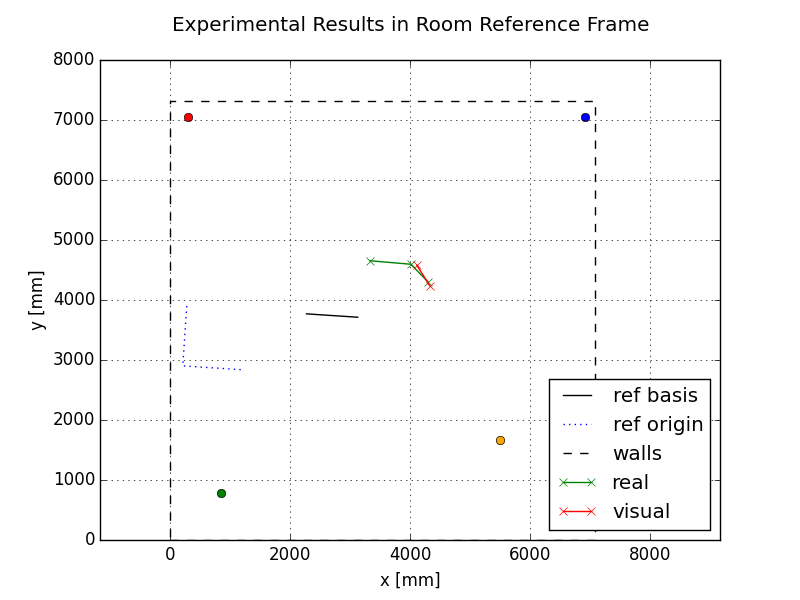
\includegraphics[width=\linewidth]{files/res2_room.png}
    \caption{Summary of results in room reference frame (Camera numbering: blue 139, red 141, green 143, orange 145)}
    \label{fig:res2_room}
\end{figure}




